\let\negmedspace\undefined
\let\negthickspace\undefined
\documentclass[journal]{IEEEtran}
\usepackage[a5paper, margin=10mm, onecolumn]{geometry}
%\usepackage{lmodern} % Ensure lmodern is loaded for pdflatex
\usepackage{tfrupee} % Include tfrupee package

\setlength{\headheight}{1cm} % Set the height of the header box
\setlength{\headsep}{0mm}     % Set the distance between the header box and the top of the text

\usepackage{gvv-book}
\usepackage{gvv}
\usepackage{cite}
\usepackage{amsmath,amssymb,amsfonts,amsthm}
\usepackage{algorithmic}
\usepackage{graphicx}
\usepackage{textcomp}
\usepackage{xcolor}
\usepackage{txfonts}
\usepackage{listings}
\usepackage{enumitem}
\usepackage{mathtools}
\usepackage{gensymb}
\usepackage{comment}
\usepackage[breaklinks=true]{hyperref}
\usepackage{tkz-euclide} 
\usepackage{listings}
% \usepackage{gvv}                                        
\def\inputGnumericTable{}                                 
\usepackage[latin1]{inputenc}                                
\usepackage{color}                                            
\usepackage{array}                                            
\usepackage{longtable}                                       
\usepackage{calc}                                             
\usepackage{multirow}                                         
\usepackage{hhline}                                           
\usepackage{ifthen}                                           
\usepackage{lscape}
\begin{document}

\bibliographystyle{IEEEtran}
\vspace{3cm}

\title{3-3.2-6}
\author{EE24BTECH11010 - Balaji}
% \maketitle
% \newpage
% \bigskip
{\let\newpage\relax\maketitle}

\renewcommand{\thefigure}{\theenumi}
\renewcommand{\thetable}{\theenumi}
\setlength{\intextsep}{10pt} % Space between text and floats

\numberwithin{figure}{enumi}
\renewcommand{\thetable}{\theenumi}

\textbf{Question :} \\
Draw a right triangle $ABC$ in which $BC$ = 12cm, $AB$ = 5cm and $\angle{B} = 90\degree$.\\
\textbf{Solution:}

\begin{table}[h!]
      \centering
      \begin{tabular}[12pt]{ |c| c| c|c|c|c|}
    \hline
    $X$ & 1 & 2 & 3 & 4 & 5 \\
    \hline
    $P(X)$ & $K$ & 2$K$ & 2$K$ & 3$K$ & $K$ \\
    \hline 
    \end{tabular} 

      \caption{}
\end{table}
Using cosine rule, we can find the length of $AC$, i.e., ${b}$:
\begin{align}
    b^2 &= a^2 + c^2 - 2ac\cos{B}\\
    b^2 &= 12^2 + 5^2 - 120\cos{90\degree}
\end{align}
On solving, we get ${b}$ as:
\begin{align}
    {b} = 13cm
\end{align}

The coordinates of $\triangle ABC$ can then be expressed as
\begin{align}
    \vec{A} = c\myvec{\cos{B} \\ \sin{B}}, \vec{B} = \myvec{0 \\ 0}, \vec{C} = \myvec{a \\ 0}
    \end{align}
    From above substituting the values of $a, b, c$, we get 
  \begin{align}
     \vec{A} = 5\myvec{\cos{90\degree} \\ \sin{90\degree}}, \vec{B} = \myvec{0 \\ 0}, \vec{C} = \myvec{ 12\\ 0} \\
    \therefore \vec{A} = \myvec{0 \\ 5}, \vec{B} = \myvec{0 \\ 0}, \vec{C} = \myvec{ 12\\ 0}   
\end{align}
\begin{figure}
    \centering
    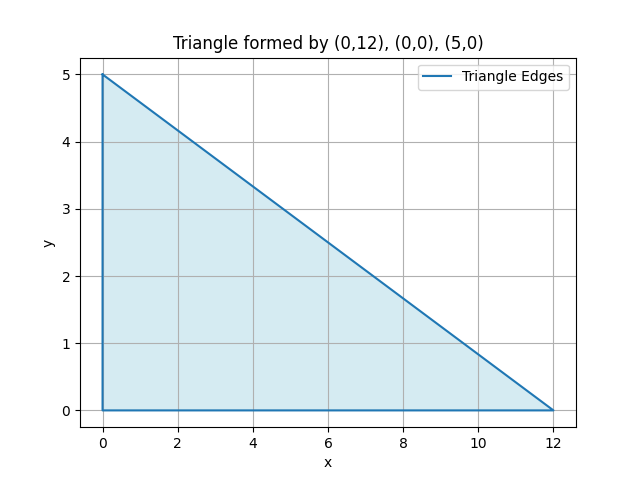
\includegraphics[width=10cm]{figs/fig.png}
    \caption{}
    \label{fig:enter-label}
\end{figure}
\end{document}
